\subsection{Aggressive Subscribers}\label{subsec:prevalence}

\begin{figure}[ht]
\begin{minipage}{1\linewidth}
\centering
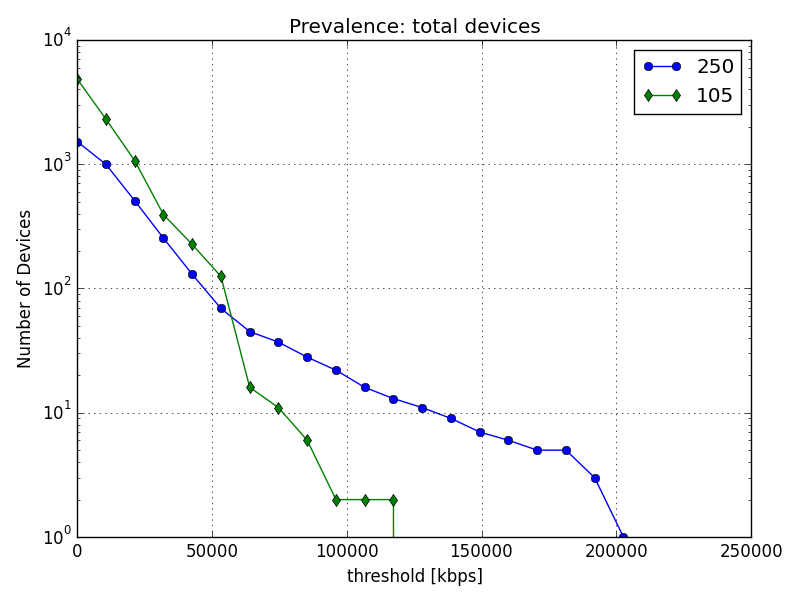
\includegraphics[width=0.9\linewidth]{figures/prevalence.png}
\caption{User prevalence as threshold increases.}
\label{fig:prevalence}
\end{minipage}
\end{figure}

\sg{Outliers. Prevalence.}
While the general behavior did not change, 11 users maxed out traffic.
For example (explain the fig: any user reaching the threshold at ANY time 
over three months). Only 2 users in the \control{} group reached high 
utilization at \textbf{any} moment. In \treatment{} 11 such users were present, 
for whom utilization over their lifetime was greater than 1 when compared to 
the 105 Mbps capacity (but lower than 250 Mbps).